\documentclass[a4paper,12pt]{report}
\usepackage{algorithmic}
\usepackage[linesnumbered,ruled,vlined]{algorithm2e}
\usepackage[margin=2cm]{geometry}
\usepackage[utf8]{inputenc}
\usepackage{listings} 
\usepackage{graphicx} 
\usepackage{color}
\usepackage{xcolor}
\usepackage{hyperref}
\usepackage{verbatim}
\usepackage{pythontex}
\usepackage{mathtools}
\usepackage{caption}
%\usepackage{mdframed}
\definecolor{codegreen}{rgb}{0,0.6,0}
\definecolor{codegray}{rgb}{0.5,0.5,0.5}
\definecolor{codepurple}{rgb}{0.58,0,0.82}
\definecolor{backcolour}{rgb}{0.95,0.95,0.92}

\lstdefinestyle{mystyle}{
    backgroundcolor=\color{backcolour},   
    commentstyle=\color{codegreen},
    keywordstyle=\color{magenta},
    numberstyle=\tiny\color{codegray},
    stringstyle=\color{codepurple},
    basicstyle=\ttfamily\footnotesize,
    breakatwhitespace=false,         
    breaklines=true,                 
    captionpos=b,                    
    keepspaces=true,                 
    numbers=left,                    
    numbersep=5pt,                  
    showspaces=false,                
    showstringspaces=false,
    showtabs=false,                  
    tabsize=2
}

\lstset{style=mystyle}

\newcommand{\currentdata}{14 February 2015}
\newtheorem{example}{Example}

\begin{document}
\vspace{-5cm}
\begin{center}
Department of Computer Science\\
Technical University of Cluj-Napoca\\

\includegraphics[width=10cm]{fig/footer}
\end{center}
\vspace{1cm}
%\maketitle
\begin{center}
\begin{Large}
 \textbf{Artificial Intelligence}\\
\end{Large}
\textit{Laboratory activity - Knight Moves on Chess Table}\\
\vspace{3cm}
Name: Tanul Gabriel-Ștefan și Pucani Liviu Cătălin\\
Group: 30232\\
Email: tus\underline{\hspace{.1in}}gabi@yahoo.com \\
       \hspace{1.70cm}liviupucani@gmail.com\\
\vspace{12cm}
Teaching Assistant: Anca Iordan\\
anca.iordan@campus.utcluj.ro\\
\vspace{1cm}


  
 
\end{center}

\tableofcontents

%\chapter{Laboratory works}
\chapter{A1: Cerință} 
    Se da o tabla de sah cu dimensiunea NxN. Un cal are initial o pozitie (xs, ys) pe tabla si trebuie sa ajunga la o pozitie de finish (xf, yf). Generati o secventa de mutari ale calului astfel incat acesta sa ajunga de la pozitia de start la cea de finish, fara a trece printr-o casuta de 2 ori.
\linebreak 
\linebreak 
\linebreak 
Stare initială – (xs, ys) \\
Stare finală – (xf, yf) \\ 
Actiuni posibile (daca tabla de sah le permite), unde (x, y) – pozitia curenta a calului \\
(x-2, y+1),(x-1, y+2),(x+1, y+2),(x+2, y+1),(x+2, y-1),(x+1, y-2),(x-1, y-2),(x-2, y-1) \\
Nivele de dificultate: N = 8, N = 12, N = 16, N = 20
\\\\\\\\
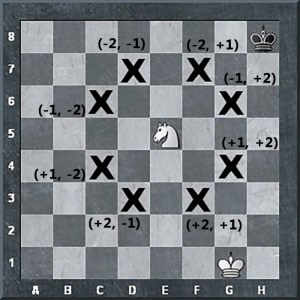
\includegraphics{problema.png}
\chapter{A2: Metode de căutare} 
 
\rule{\textwidth}{0.5pt}
\section{Breadth First Search}
Căutarea (parcurgerea) în lățime (BFS) este un algoritm pentru parcurgerea sau căutarea într-o structură de date de tip arbore sau graf. Aceasta începe cu rădăcina arborelui (sau cu un nod arbitrar dintr-un graf, uneori denumit "cheie de căutare") și explorează nodurile mai întâi nodurile vecine acestuia, înainte de a trece la vecinii de pe nivelul următor (vecinii vecinilor).\\

\section{Depth First Search}
Căutarea sau parcurgerea în adâncime (denumită și ca în engleză depth-first search, abreviat DFS) este un algoritm pentru parcurgerea sau căutarea într-o structură de date de tip arbore sau graf. Se începe de la rădăcină (sau alegând un nod arbitrar ca rădăcină în cazul unui graf) și se explorează cât mai mult posibil de-a lungul fiecărei ramuri înainte de a face pași înapoi.
\section{Uniform Cost Search}
Căutarea folosind costuri uniforme (UCS) este un algoritm de căutare pe arbori utilizat pentru parcurgerea sau căutarea unui arbore ponderat, a unei structuri de arbore sau a unui grafic. În mod intuitiv, căutarea începe de la nodul rădăcină și continuă vizitând următorul nod care are cel mai mic cost total de la rădăcină. Nodurile sunt vizitate în acest mod până când se atinge o stare finală dorită.
\section{A* Star Search}
A* este un algoritm de parcurgere a grafului și de căutare a căii, care este adesea folosit în multe domenii ale informaticii datorită completitudinii, optimității și eficienței optime.
A* este un algoritm de căutare informată, ceea ce înseamnă că este formulat în termenii grafurilor cu ponderi: pornind de la un anumit nod de start al unui graf, se urmărește calea către nodul obiectiv dat având cel mai mic cost (cea mai mică distanță parcursă, cel mai scurt timp etc.) adică o euristică. Face acest lucru menținând un arbore de căi care provin de la nodul de pornire și extinzând acele căi câte o muchie până când criteriul său de terminare este îndeplinit.
 \subsection{Euristica Manhattan}
 Distanța Manhattan este o distanță specifică într-o geometrie în care funcția obișnuită de distanță (metrică) din geometria euclidiană este înlocuită cu o nouă metrică în care distanța dintre două puncte este suma diferențelor absolute ale coordonatelor carteziene. Metrica Manhattan este cunoscută și ca distanță L1, distanță L1 sau normă. Denumirea distanței provine de la trama stradală din Manhattan, unde traseele taximetrelor pot avea aceeași lungime pentru diferite căi.
  \begin{lstlisting}[language=Python]
def manhattanDistance(state, finalX, finalY):
    currentX, currentY = state
    return (abs(currentX - finalX) + abs(currentY - finalY)) / 3
\end{lstlisting}
 \subsection{Euristica de potrivire a culorilor}
 Observăm că un cal se poate muta doar în pătrate colorate opuse (deci de la negru la alb sau alb la negru) și am decis să proiectăm o euristică în jurul acestui lucru. Dacă următoarea stare este de altă culoare, îi atribuim a cost de 1, în caz contrar 2.  
 Este nevoie de minimum 1 mișcare pentru a ajunge la o stare de obiectiv și un minim de 2 mișcări când obiectivul starea este de aceeași culoare.
 Deci costul la obiectiv nu este niciodată supraestimat. În plus, euristica nodului curent va fi întotdeauna mai mică decât sau egală cu euristica unui nod vecin plus costul deplasării la acel nod (este nevoie de o mișcare pentru a ajunge la vecin).
  \begin{lstlisting}[language=Python]
 def matchingColors(state, finalX, finalY):
    """
    A heuristic function estimates the cost from the current state to the nearest
    goal in the provided SearchProblem.  This heuristic is trivial.
    """
    currentX, currentY = state
    auxX = currentX % 2
    auxY = currentY % 2
    aux2X = finalX % 2
    aux2Y = finalY % 2
    if auxX == aux2X and auxY == aux2Y:
        return 2
    elif auxX == aux2X and auxY != aux2Y:
        return 1
    elif auxX != aux2X and auxY == aux2Y:
        return 1
    elif auxX != aux2X and auxY != aux2Y:
        return 2 
\end{lstlisting}   
\rule{\textwidth}{0.5pt}
 

\chapter{A3: Comparare metode}
 Am ales pentru testarea algoritmilor mereu starea inițială a piesei (0,0) și starea finală colțul opus al tablei de șah ( (7,7), (11,11), (15,15), (19,19)).
 \\În primă fază am testat algoritmul DFS și am ajuns la concluzia că nu este cel mai eficient algoritm de determinare al celui mai scurt drum dintre starea inițială și starea finală deoarece parcurge în adâncime tabla și expandează multe noduri.\\
 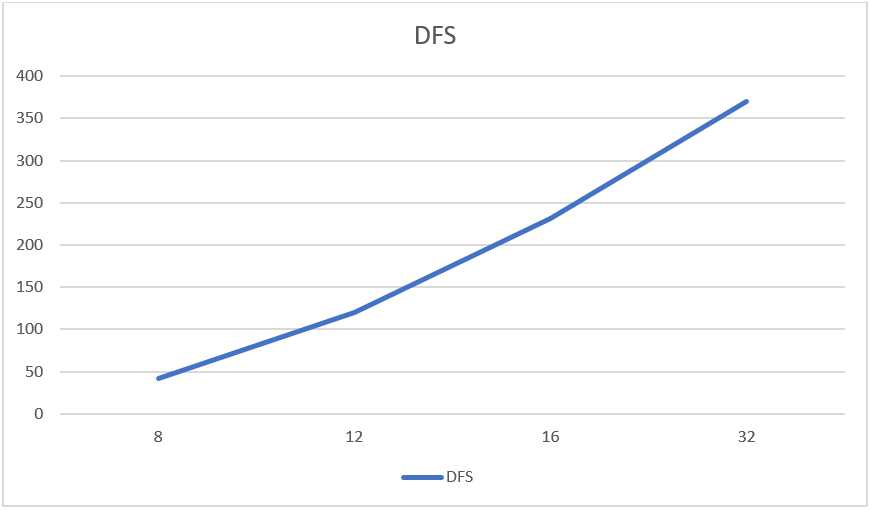
\includegraphics{fig/DFS.PNG}\\
 \\\\\\\\\\\\\\\\\\\\\\\\\\\\\\\
 În cazul algoritmului BFS situația se schimbă și parcurgerea drumului se realizează pe o cale minimă.\\
 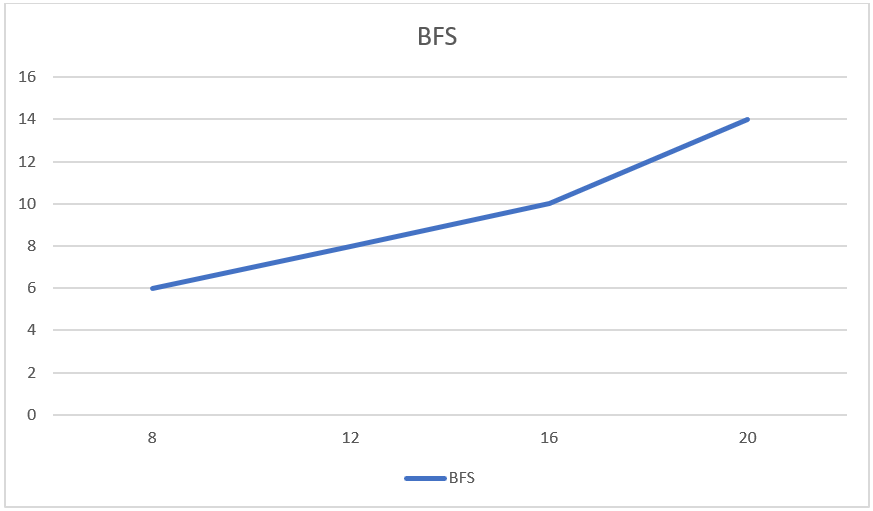
\includegraphics{fig/BFS.PNG}
 
 De asemenea pentru algoritmul UCS se observă o diferență în cazul introducerii nodurilor expandate în coadă deoarece se folosește o coadă de priorități după costul unei mutări. Se calculează drumul minim.\\
 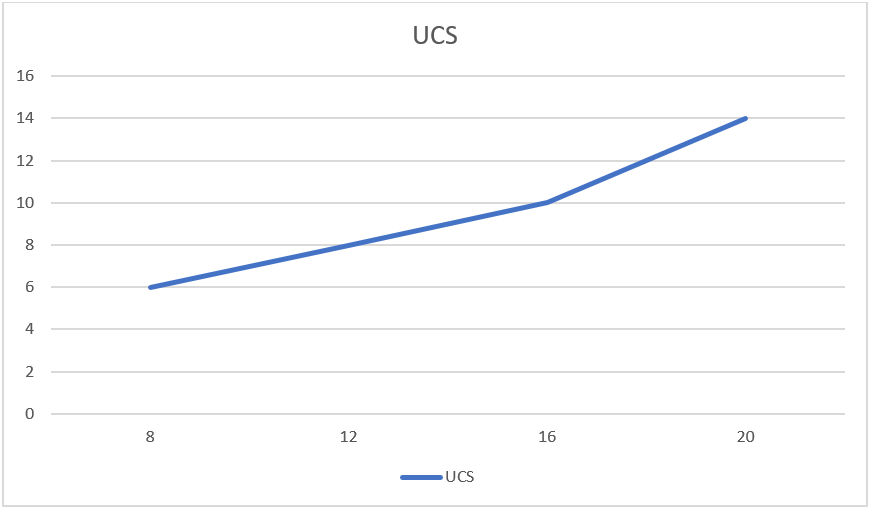
\includegraphics{fig/UCS.PNG}
 
 Algoritmul A* Search folosește de asemenea o coadă de priorități însă de data aceasta condiția de prioritate depinde de o euristică implementată de noi.\\
 Pentru euristica Manhattan se calculează drumul minim bazat pe diferenta de coordonate dintre starea curentă și starea finală.\\
 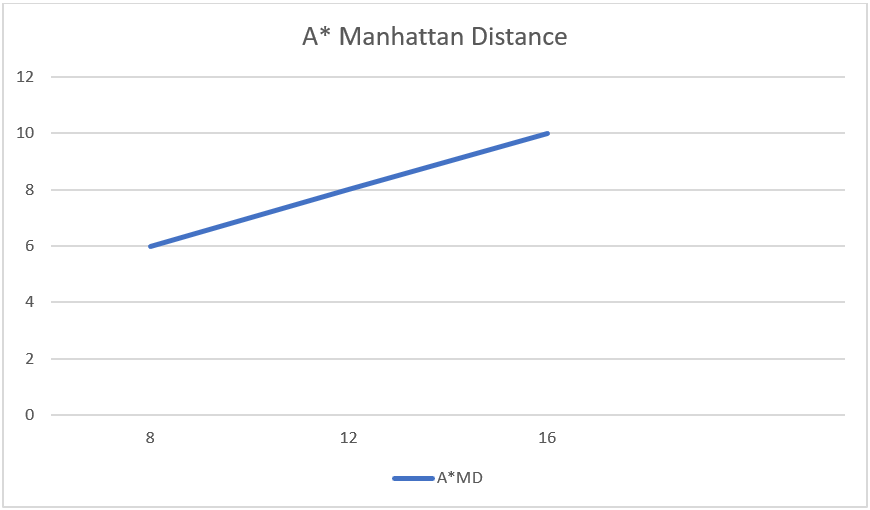
\includegraphics{fig/ASSMD.PNG}
 
 Pentru euristica potrivirii culorilor se calculează drumul minim bazat pe costul ales în funcție de starea curentă și starea finală influențat de culoarea căsuței pe care se află calul pe tabla de șah.\\
 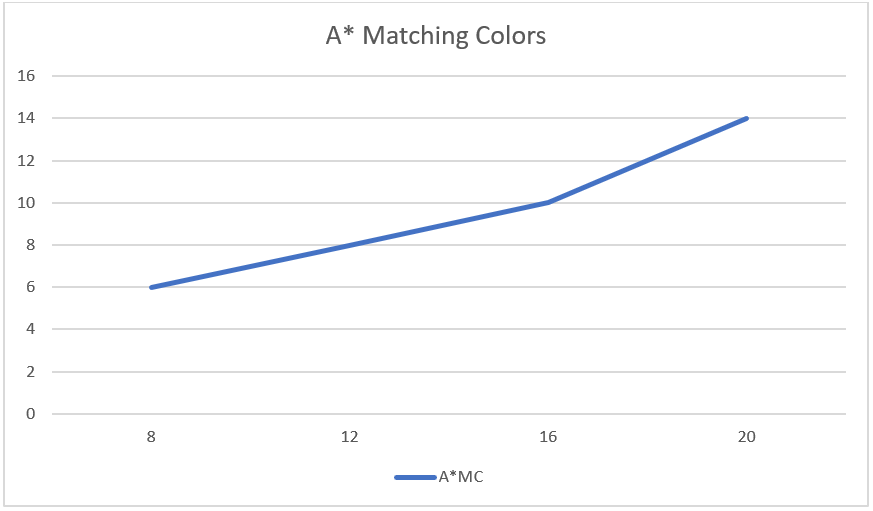
\includegraphics{fig/ASSMC.PNG}
\bibliographystyle{plain}
\bibliography{is}  
\url{https://www.overleaf.com/learn} \\
\url{https://ro.wikipedia.org/wiki/C%C4%83utare_%C3%AEn_ad%C3%A2ncime} \\
\url{https://ro.wikipedia.org/wiki/C%C4%83utare_%C3%AEn_l%C4%83%C8%9Bime} \\
\url{https://en.wikipedia.org/wiki/A*_search_algorithm}
\url{https://ro.wikipedia.org/wiki/Distan%C8%9B%C4%83_Manhattan}
\url{https://en.wikipedia.org/wiki/Pygame}
\url{https://www.pygame.org/tags/all}
\appendix

\chapter{Codul folosit în implementare}
 BFS\\
\begin{lstlisting}[language=Python]
def breadthFirstSearch(finalX, finalY, boardSize):
    visited = set()
    queue = util.Queue()
    duplicates = []
    queue.push(((0, 0), list()))
    listActions = []
    while not queue.isEmpty():
        currentPos = queue.pop()

        currentX, currentY = currentPos[0]
        if currentX == finalX and currentY == finalY:
            print("The list of actions is: ", currentPos[1])
            return currentPos[1]
        else:
            successors = getActions(currentPos[0], boardSize)
            visited.add(currentPos[0])
            for successor in successors:
                if successor[0] not in visited and successor[0] not in duplicates:
                    listActions = list(currentPos[1])
                    listActions.append(successor[1])
                    queue.push((successor[0], listActions))
                    duplicates.append(successor[0])

    return listActions 

\end{lstlisting} 

   DFS\\
\begin{lstlisting}[language=Python]
def depthFirstSearch(finalX, finalY, boardSize):
    visited = set()
    stack = util.Stack()
    stack.push(((0, 0), list()))
    listActions = []
    while not stack.isEmpty():
        currentPos = stack.pop()
        currentX, currentY = currentPos[0]
        if currentX == finalX and currentY == finalY:
            print("The list of actions is: ", currentPos[1])
            return currentPos[1]
        else:
            successors = getActions(currentPos[0], boardSize)
            visited.add(currentPos[0])
            for successor in successors:
                if successor[0] not in visited:
                    listActions = list(currentPos[1])
                    listActions.append(successor[1])
                    stack.push((successor[0], listActions))

    return listActions

\end{lstlisting} 
UCS\\
\begin{lstlisting}[language=Python]
def uniformCostSearch(finalX, finalY, boardSize):
    """Search the node of least total cost first."""
    "*** YOUR CODE HERE ***"
    visited = []
    queue = util.PriorityQueue()
    start = (0, 0)
    queue.push((start, [],0), 0)
    while not queue.isEmpty():
        currentPosition = queue.pop()
        currentState = currentPosition[0]
        currentX, currentY = currentPosition[0]
        path = currentPosition[1]
        if currentX == finalX and currentY == finalY:
            print("The list of actions is: ",currentPosition[1],"\nThe cost is",currentPosition[2])
            return currentPosition[1]
        if currentState not in visited:
            visited.append(currentState)
            successorsList = getActions(currentState, boardSize)
            for successor in successorsList:
                if successor[0] not in visited and successor[0] not in [nod[0] for nod in queue.heap]:
                    currentRoute = list(path)
                    currentRoute += [successor[1]]
                    cost = currentPosition[2]
                    queue.push((successor[0], currentRoute, cost + 1), cost + 1)


\end{lstlisting} 
A* Search\\
   
\begin{lstlisting}[language=Python]
def aStarSearchMC(finalX, finalY, boardSize, heuristic=matchingColors):
    """Search the node that has the lowest combined cost and heuristic first."""
    "*** YOUR CODE HERE ***"
    visited = []
    queue = util.PriorityQueue()
    start = (0, 0);

    startHeuristic = heuristic(start, finalX, finalY)
    queue.push((start, [], startHeuristic),startHeuristic)

    while not queue.isEmpty():
        currentPosition = queue.pop()
        currentState = currentPosition[0]
        currentX, currentY = currentPosition[0]
        if currentX == finalX and currentY == finalY:
            print("The list of actions is: ",currentPosition[1],"\nThe cost is",currentPosition[2])
            return currentPosition[1]
        if currentState not in visited:
            visited.append(currentState)
            successorsList = getActions(currentState, boardSize)
            for successor in successorsList:
                if successor[0] not in visited and successor[0] not in [nod[0] for nod in queue.heap]:
                    currentRoute = list(currentPosition[1])
                    currentRoute += [successor[1]]
                    cost = currentPosition[2]
                    getHeuristic = heuristic(successor[0], finalX, finalY)
                    queue.push((successor[0], currentRoute,  cost + getHeuristic),cost + getHeuristic)

    return []
\end{lstlisting}
\vspace{2cm}
\begin{center}


\includegraphics[width=10cm]{fig/footer}
\end{center}



\end{document}
